\section{Discussion}
\label{sec:discussion}
results that are contradictory\\
results that data suggests that is wrong\\ 
- suggest that this may be due to representation\\
a better way to measure and offer broadband based on utilization?

\subsection{User Taxonomy}
\label{subsec:taxonomy}


\todo{This splitting needs to be done}

\begin{figure}[t!]
\begin{minipage}{1\linewidth}
\centering
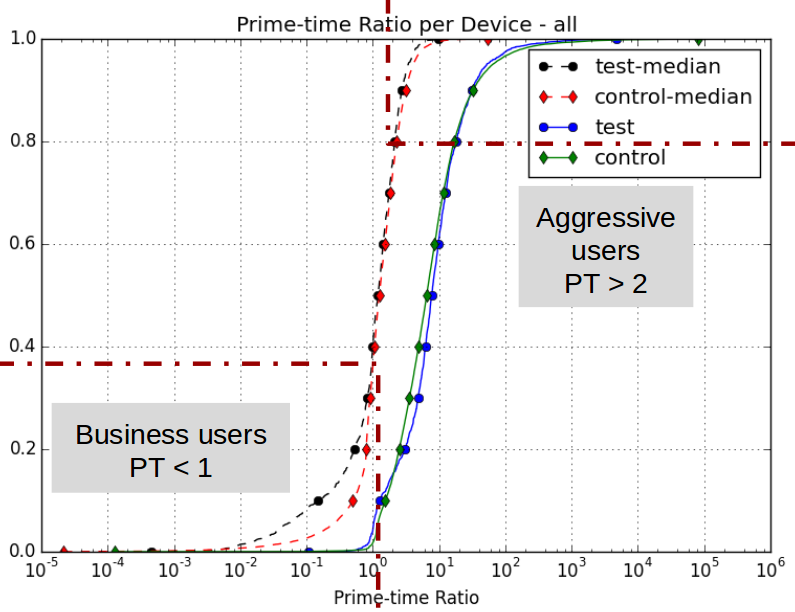
\includegraphics[width=\linewidth]{figures/cdf-prime-time-ratio[replace].png}
\caption{(old) Prime Time ratio + usage can be used to divide users into four sets: aggressive all time + non aggressive all time, aggressive peak time, aggressive non-peak time (business hours))}
%http://riverside.noise.gatech.edu:8083/separated/full/cdf-prime-time-ratio-per-device.png\\
%http://riverside.noise.gatech.edu:8083/plots/full_dw/prime-time-ratio-per-device-cdf-ALL.png
\label{fig:CDF-prime-time-ratio}
\end{minipage}
\end{figure}




% peak ratio cdf vs no of devices
% peak ratio cdf vs time of day where peak occured
% no of devices cdf vs time of day where peak occured
